Nesta seção são descrevemos em detalhes a implementação aplicada ao \textit{benchmark} Bench4Q e como ele pode ser estendido. Descrevemos também algumas das complexidades na produção de distribuições para a carga de trabalho. Essa ferramenta também está disponível sob uma licença de código aberto, para que outros possam usar e estender o \textit{benchmark}, e contribuir com novos tipos de modulação de cargas de trabalho. O código fonte esta disponível em \href{URL}{http://gitlab.lasdpc.icmc.usp.br/edwin/bench4q}. A Figura \ref{fig:diagrama-classes} mostra o diagrama de classes envolvido na extensão do Bench4Q. As classes sinalizadas na cor azul, representam as já existentes mas que passaram por adaptações e modificações, já as classes na cor verde, referem-se as novas classes criadas para possibilitar a modulação da carga do \textit{benchmark}.

Apesar de permitir a geração de carga para o sistema SUT, o Bench4Q possui algumas limitações na sua versão original que dificultam a experimentação e analise de cenários de interesse ao trabalho de \citeonline{Edwin2015} e \citeonline{Lourenco2015}.
As classes disponíveis no \textit{benchmark} original não permitem a modulação de carga de trabalho. Essa limitação implica, por exemplo, na dificuldade de projetar um controlador para o gerenciamento de recursos, pois para esta atividade é necessário uma análise de resultados transientes mediante a modulação da carga de trabalho. A simulação de uma carga de trabalho em que há a alteração introduzida ao longo da simulação é o foco deste trabalho.

O modelo de referencia MEDC define um conjunto de requisitos a qual esta extensão deve seguir e respeitar o requisito \textit{Demand}. Segundo \citeonline{Edwin2015}, o requisito \textit{Demand} visa a avaliação de desempenho de sistemas computacionais considerando mudanças na carga de trabalho que chega ao sistema. Para o contexto do Bench4Q, a carga de trabalho são requisições Web que são submetidas à camada de aplicação. 

O Console do Bench4Q é um programa Java que gerencia EBs para gerar uma série sequencial programada de requisições a serem enviadas para o SUT. 
Os tópicos aqui é controlar a taxa em que os EBs geram as requisições, para que seja possível controlar diretamente, de forma programada, a carga de trabalho oferecida para o SUT. Nativamente o Bench4Q, coleta informações sobre a taxa requisições e o comportamento do SUT, e relata esses dados no final da experimento. A Figura \ref{fig:experimental-setup} ilustra este contexto.

\begin{figure}[!htb]
	\centering
	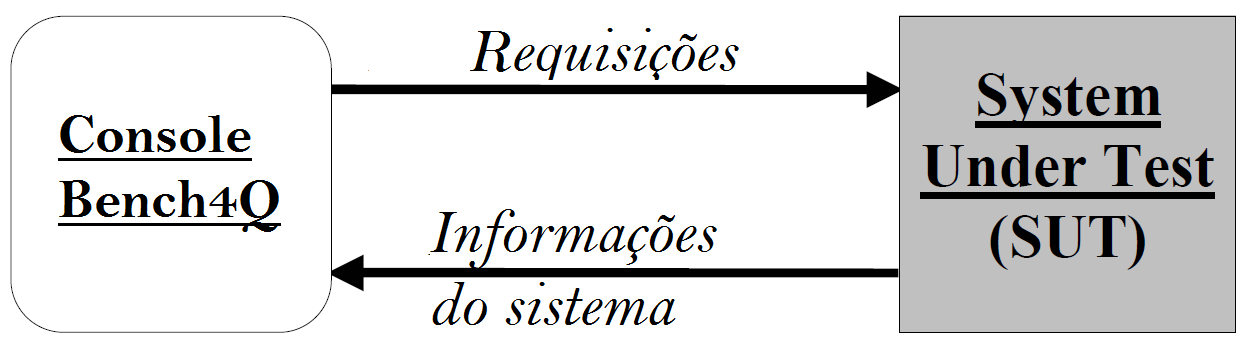
\includegraphics[scale=0.6]{experimental-setup.png}	
	\caption{Configuração experimental Bench4Q.}
	\label{fig:experimental-setup}
	\fadaptada{Vieira2003}
\end{figure}

A extensão implementada na geração de carga do Bench4Q segue a orientação do requisito \textit{Demand} do MEDC, modificando algumas classes da versão original do \textit{benchmark}. Conforme o diagrama de classes na Figura \ref{fig:diagrama-classes}, é possível ter uma ideia do trabalho de extensão realizado no \textit{benchmark}. Vale  salientar que o Bench4Q é uma ferramenta completa e extensa, e diagramar todas as suas classes seria difícil e aumentaria consideravelmente a complexidade de entendimento. Sendo assim, aqui apresentamos somente as classes já existem no Bench4Q e que passaram por modificações para atender aos requisitos da proposta, juntamente com as novas classes que foram necessárias para o mesmo objetivo.
 
O Bench4Q fornece uma estrutura e componentes compartilhados para a comunicação entre os dois módulos da carga de trabalho: \textbf{Console} e \textbf{Agente}. Apesar de trabalharem em conjunto e para um mesmo fim, os módulos (Console e Agente) são executados em máquinas distintas.  A extensão é construída inicialmente sob a classe \textsf{MLoadSimulatorPanel}, que orquestra toda a interatividade gráfica do Bench4Q. O novo painel de configuração, que modula a carga, \textsf{MLoadFrequencyPanel} estende da classe original \textsf{Bench4QTreeModel}, adicionando os parâmetros para a modulação: tipo da carga, o instante em que a carga se inicia, o tempo de atuação da carga e a quantidade de EBs que atuaram nessa carga. O parâmetro \textit{"tipos de carga"}, utiliza da classe enum \textsf{TypeFrequency} que define as constantes dos tipos de modulações programadas para esta extensão.  Todos os parâmetros inseridos na \textsf{MLoadSimulatorPanel} são armazenados na classe \textsf{TestFrequency} que se tornou uma propriedade da classe nativa \textsf{TestPhase}, e que posteriormente são repassadas para a classe \textsf{PropertiesEB} através da \textsf{FrequencySettings}. Já as classes \textsf{Agent}, \textsf{EB}, \textsf{EBClose}, \textsf{EBOpen}, \textsf{Workers}, \textsf{WorkersClosed} e \textsf{WorkersOpen} foram modificadas para receber os novos parâmetros da \textsf{PropertiesEB} e compreendê-los correspondentemente a modulação configurada na interface gráfica, gerando a carga programada durante a execução.
 
\begin{figure}[!htb]
	\centering
	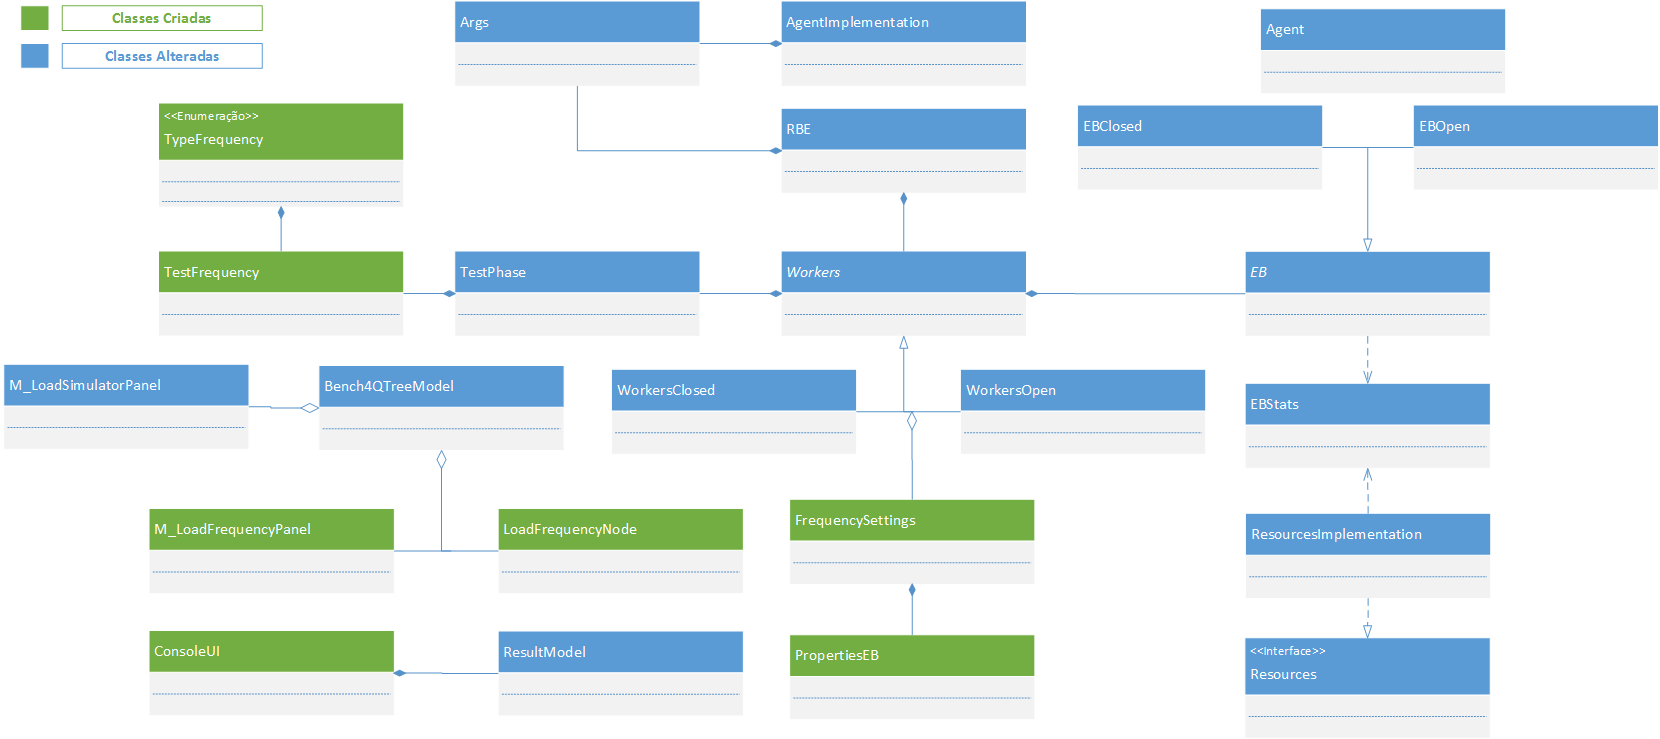
\includegraphics[angle=90, scale=0.6]{diagrama-classes-beanch4Q.png}	
	\caption{Diagrama de classes da extensão do Bench4Q.}
	\label{fig:diagrama-classes}
	\fautor
\end{figure}

O trabalho de desenvolver a extensão compreendeu extensivas modificações no código-fonte original do Bench4Q e a criação de novas funcionalidades. Por conta de espaço e clareza não cabe uma descrição minuciosa de todas as alterações feitas. Resumem-se, apenas, algumas das principais intervenções realizadas.

\section{Configuração da carga de trabalho}
O Agente do Bench4Q é um cliente conectado ao modulo Console do \textit{benchmark}, a ferramenta permite que diversos clientes em diferentes máquinas estejam conectados em um mesmo Console.
O Cliente é um programa Java para gerar as operações que compõem a carga de trabalho. Cada \textit{thread} executa uma série sequencial de operações, fazendo chamadas para o SUT. Para distribuir e controlar a submissão da carga de trabalho ao longo da simulação, uma estratégia utilizada é a modulação da mesma através de parâmetros que configuram o comportamento da carga. O cliente tem uma série de propriedades que definem o seu funcionamento e o comportamento resultante da carga de trabalho, apresentados no Capítulo \ref{chapter:metodologia}. 

O código \ref{code:createProperties} apresentado na integra, esta presente na classe \textit{FrequencySettings} criada para a extensão, que contém o algoritmo responsável por calcular os tempos de inicialização, pause e termino de cada um dos clientes. Este código é ponto central que resulta no comportamento final da modulação da carga de trabalho.

\begin{codigo}[caption={Algoritmo calcula os tempos de iniciaçização e termino para cada um dos Clientes}, label={code:createProperties}, breaklines=true]
	public static PropertiesEB createProperties(int index, TestPhase testPhase, TypeFrequency type, long beginTime) {
		
		PropertiesEB propertiesEB = new PropertiesEB();
		Logger.getLogger().debug(type.getName());
		propertiesEB.isFrenquency = true;
		propertiesEB.setIndexEB(index);
		
		long timeStart = testPhase.getFrequency().getStartTime() * 1000 + beginTime;
		long timeEnd   = testPhase.getFrequency().getEndTime() * 1000 + timeStart;
		long timePause = testPhase.getFrequency().getPauseTime() * 1000;
		long timeExperiment = testPhase.getExperimentTime() * 1000 + beginTime;
		
		if (TypeFrequency.STEP.equals(type)) {
			if (index >= testPhase.getFrequency().getQuantity()) {
				propertiesEB.setStartTime(beginTime);
				propertiesEB.setEndTime(timeExperiment);
				propertiesEB.setEndExperimentTime(timeExperiment);
				Logger.getLogger().debug("Normal: " + index);
			} else {
				propertiesEB.setStartTime(timeStart);
				propertiesEB.setEndTime(timeEnd);
				propertiesEB.setEndExperimentTime(timeExperiment);
				Logger.getLogger().debug("To Step: " + index);
			}
		} else if (TypeFrequency.PULSE.equals(type)) {
			if (index >= testPhase.getFrequency().getQuantity()) {
				propertiesEB.setStartTime(beginTime);
				propertiesEB.setEndTime(timeExperiment);
				propertiesEB.setEndExperimentTime(timeExperiment);
				Logger.getLogger().debug("Normal: " + index);
			} else {
				propertiesEB.setStartTime(timeStart);
				propertiesEB.setPauseTime(timePause);
				propertiesEB.setEndTime(timeEnd);
				propertiesEB.setEndExperimentTime(timeExperiment);
				Logger.getLogger().debug("To Pulse: " + index);
			}
		}

		return propertiesEB;

	}

\end{codigo}
A verdade é que motivamos em tornar mais fácil a contribuição de novas variedades de carga de trabalho para outros desenvolvedores. Logo, as novas modulações a serem implementadas deve ser incluídas neste método, juntamente com o nome da nova carga na classe Enum \textit{TypeFrequency}.


\section{Geração da carga de trabalho}
A princípio foi identificado o modulo de geração de carga do Bench4Q e este passou por alterações para gerar a carga de trabalho esperada. Logo, esta classe é nativa do \textit{benchmark}. O Bench4Q tem dois tipos de conexões, \textit{Open}(Aberta) e \textit{Close}(Fechada), consequentemente existem duas classes que tratam cada umas das conexões (\textit{WorkersOpen} e \textit{WorkersClose}) com o mesmo métodos, mas com programações diferentes.
O código-fonte \ref{code:modelworkload}, apresentado na integra, ilustra o \textit{core} da geração da carga referente a construção da modulação da carga já com as modificações da extensão, este método é o manipula as conexões geradas pelos clientes. Através dos parâmetros e dados calculados anteriormente é possível controlar as requisições afim de gerar as modulação deseja.

\begin{codigo}[caption={Algoritmo de geração de carga modificado para modulação}, label={code:modelworkload}, breaklines=true]
public void test() {
	long tt = 0L; // Think Time.
	boolean sign = true;
	long startGet = System.currentTimeMillis();
	long currentTimeMillis = System.currentTimeMillis();
	this.sessionStart = startGet;
		
		
	while ((this.maxTrans == -1) || (this.maxTrans > 0)) {
			
		//avaliando o EB segundo o tempo percorrido do experimento
		currentTimeMillis = System.currentTimeMillis();
		
		if (currentTimeMillis > this.propertiesEB.getEndExperimentTime()){
			Logger.getLogger().debug(propertiesEB.getIndexEB() + " is stopping ... " + (currentTimeMillis - startExp)/1000);
			this.test = false;
		}
			
		if (currentTimeMillis > this.propertiesEB.getEndTime() && this.propertiesEB.isFrenquency()) {
			//desactivado = -1
			if(this.propertiesEB.getPauseTime() > 0){
				long newInit = this.propertiesEB.getEndTime() + this.propertiesEB.getPauseTime();
				long period = this.propertiesEB.getEndTime() - this.propertiesEB.getStartTime();
				
				this.propertiesEB.setStartTime(newInit);
				this.propertiesEB.setEndTime(period + newInit);
				
				Logger.getLogger().debug(propertiesEB.getIndexEB() + " was restarted  ... ");
			}else{
				Logger.getLogger().debug(propertiesEB.getIndexEB() + " is ending ... " + (currentTimeMillis - startExp)/1000);
				this.test = false;
			}
		}
		
		// alguns EBs nao iniciam inmediatamente, porque foram marcados para esperar
		if (currentTimeMillis >= this.propertiesEB.getStartTime()) {
			if (this.terminate || !this.test) {
				this.sessionEnd = System.currentTimeMillis();
				EBStats.getEBStats().sessionRecorder(this.sessionStart, this.sessionEnd, this.sessionLen,
				this.Ordered, this.isVIP);
				return;
			}
				
			long endGet;
			if (this.nextReq != null) {
				// Check if user session is finished.
				if (this.toHome) {
					// User session is complete. Start new user session.
					this.sessionEnd = System.currentTimeMillis();
					EBStats.getEBStats().sessionRecorder(this.sessionStart, this.sessionEnd, this.sessionLen,
					this.Ordered, this.isVIP);
					initialize();
					return;
				}
				if (this.nextReq.equals("")) {
					EBStats.getEBStats().addErrorSession(this.curState, this.isVIP);
					initialize();
					continue;
				}
				// Receive HTML response page.
				if (this.rate > 0) {
					if (isVIP) {
						if (this.nextReq.contains("?")) {
							this.nextReq += "&bench4q_session_priority=10";
						} else {
							this.nextReq += "?bench4q_session_priority=10";
						}
					} else if (this.nextReq.contains("?")) {
						this.nextReq += "&bench4q_session_priority=1";
					} else {
						this.nextReq += "?bench4q_session_priority=1";
					}
				}

			// additional load
			if(this.addLoad > 0 && this.addLoadOpt >= 0) {
				if (this.nextReq.contains("?")) {
					this.nextReq += "&bench4q_add_load=" + this.addLoad + "&bench4q_add_load_opt=" +this.addLoadOpt;
				} else {
					this.nextReq += "?bench4q_add_load=" + this.addLoad + "&bench4q_add_load_opt=" +this.addLoadOpt;
				}
			} else {
				if (this.nextReq.contains("?")) {
					this.nextReq += "&bench4q_add_load=0&bench4q_add_load_opt=0";
				} else {
					this.nextReq += "?bench4q_add_load=0&bench4q_add_load_opt=0";
				}
			}

			if (this.first) {
				this.m_Client = HttpClientFactory.getInstance();
				this.m_Client.getParams().setCookiePolicy(CookiePolicy.RFC_2965);
			}

			startGet = System.currentTimeMillis();
			sign = getHTML(this.curState, this.nextReq, (currentTimeMillis - startExp)/1000);	

			endGet = System.currentTimeMillis();

			if (!sign) {
				EBStats.getEBStats().addErrorSession(this.curState, this.isVIP);
				initialize();
				
				continue;
			}
			this.first = false;

			// Compute and store Web Interaction Response Time (WIRT)
			EBStats.getEBStats().interaction(this.curState, startGet, endGet, tt, this.isVIP);
			this.sessionLen++;
			if (this.curState == 4) {
				this.Ordered = true;
			}
			this.curTrans.postProcess(this, this.html);
			} else {
				this.html = null;
				endGet = startGet;
			}

			if (!nextState()) {
				return;
			}
			if (this.nextReq != null) {
				// Pick think time (TT), and compute absolute request time
				tt = MAP();
				startGet = endGet + tt;
				if ((this.terminate) || (!this.test)) {
					return;
				}
				try {
					sleep(tt);
				} catch (InterruptedException inte) {
					Thread.currentThread().interrupt();
					return;
				}
				if (this.maxTrans > 0) {
					this.maxTrans--;
				}
			} else {
				EBStats.getEBStats().addErrorSession(this.curState, this.isVIP);
				initialize();
			}
		} else {
			try {
				// libera de sobrecarga
				Thread.sleep(500L);
			} catch (InterruptedException e) {
				// TODO Auto-generated catch block
				e.printStackTrace();
			}
		}

	}
}
\end{codigo}


\section{\textit{Interface} gráfica}

No console principal do Bench4Q, onde configura-se a execução do experimento, foi incluída uma nova opção \textit{LoadFrequency} referente ao parâmetros da extensão da geração da carga modulada. Por esta opção, \textit{LoadFrequency}, deve-se preencher os campos (\textit{Start Time}, \textit{Duration Step}, \textit{Pause} e \textit{Quantity}) que irão gerar a carga modulada conforme a programação. O código fonte \ref{code:panel} apresenta o método \textit{private} presente na classe \textit{MLoadFrequencyPanel} que cria a \textit{interface} gráfica gerada com a biblioteca \textit{Swing} do Java, toda a parte gráfica do Bench4Q utiliza da mesma biblioteca. Todos os resultados de desempenho de cada agente de carga são agregados no console de carga para análise e demonstração, conforme a versão original.

\begin{codigo}[caption={Código para gerar a os parâmetros para a modulação}, label={code:panel}, breaklines=true]
	private void createPanelFunction(final TypeFrequency type) {
		
		this.functionPanel.removeAll();
		this.m_configModel.getArgs().setTypeFrenquency(type.getName());
		int row = 0;
		
		lb_startTime = new JLabel("Start Time");
		tf_startTime = new JTextField(String.valueOf(dataSet.get(0).getFrequency().getStartTime()));
		tf_startTime.getDocument().addDocumentListener(new StartTimeListener());
		functionPanel.add(lb_startTime, new GridBagConstraints(0, row, 1, 1, 0.0, 0.0, GridBagConstraints.EAST,
		GridBagConstraints.NONE, new Insets(5, 5, 5, 5), 1, 1));
		functionPanel.add(tf_startTime, new GridBagConstraints(1, row++, 1, 1, 100.0, 0.0, GridBagConstraints.WEST,
		GridBagConstraints.HORIZONTAL, new Insets(5, 5, 5, 5), 1, 1));
		
		lb_endTime = new JLabel("Duration Step");
		tf_endTime = new JTextField(String.valueOf(dataSet.get(0).getFrequency().getEndTime()));
		tf_endTime.getDocument().addDocumentListener(new EndTimeListener());
		functionPanel.add(lb_endTime, new GridBagConstraints(0, row, 1, 1, 0.0, 0.0, GridBagConstraints.EAST,
		GridBagConstraints.NONE, new Insets(5, 5, 5, 5), 1, 1));
		functionPanel.add(tf_endTime, new GridBagConstraints(1, row++, 1, 1, 100.0, 0.0, GridBagConstraints.WEST,
		GridBagConstraints.HORIZONTAL, new Insets(5, 5, 5, 5), 1, 1));
		
		if (type.getName().compareTo("Pulse") == 0) {
			lb_pauseTime = new JLabel("Pause");
			tf_pauseTime = new JTextField(String.valueOf(dataSet.get(0).getFrequency().getPauseTime()));
			tf_pauseTime.getDocument().addDocumentListener(new PauseTimeListener());
			functionPanel.add(lb_pauseTime, new GridBagConstraints(0, row, 1, 1, 0.0, 0.0, GridBagConstraints.EAST,
			GridBagConstraints.NONE, new Insets(5, 5, 5, 5), 1, 1));
			functionPanel.add(tf_pauseTime, new GridBagConstraints(1, row++, 1, 1, 100.0, 0.0, GridBagConstraints.WEST,
			GridBagConstraints.HORIZONTAL, new Insets(5, 5, 5, 5), 1, 1));
		}
		
		if (type.getName().compareTo("Step") == 0) {
			lb_polarity = new JLabel("Polarity");
			tf_polarity = new JTextField(String.valueOf(dataSet.get(0).getFrequency().getPolarity()));
			tf_polarity.getDocument().addDocumentListener(new PolarityListener());
			functionPanel.add(lb_polarity, new GridBagConstraints(0, row, 1, 1, 0.0, 0.0, GridBagConstraints.EAST,
			GridBagConstraints.NONE, new Insets(5, 5, 5, 5), 1, 1));
			functionPanel.add(tf_polarity, new GridBagConstraints(1, row++, 1, 1, 100.0, 0.0, GridBagConstraints.WEST,
			GridBagConstraints.HORIZONTAL, new Insets(5, 5, 5, 5), 1, 1));
		}
		
		lb_quantity = new JLabel("Quantity");
		tf_quantity = new JTextField(String.valueOf(dataSet.get(0).getFrequency().getQuantity()));
		tf_quantity.getDocument().addDocumentListener(new QuantityListener());
		functionPanel.add(lb_quantity, new GridBagConstraints(0, row, 1, 1, 0.0, 0.0, GridBagConstraints.EAST,
		GridBagConstraints.NONE, new Insets(5, 5, 5, 5), 1, 1));
		functionPanel.add(tf_quantity, new GridBagConstraints(1, row++, 1, 1, 100.0, 0.0, GridBagConstraints.WEST,
		GridBagConstraints.HORIZONTAL, new Insets(5, 5, 5, 5), 1, 1));
		
		this.functionPanel.updateUI();
		this.functionPanel.repaint();
		
	}
\end{codigo}

Este conjunto de classes as quais lidam, manipulam, gerenciam e modulam a carga de trabalho gerada pelo Bench4Q, utiliza de um console para configurar, monitorar e analisar todo o experimento. Todo o desenvolvimento, referente à modificação e implementação de novas classes, mantiveram e respeitaram o padrão de desenvolvimento do \textit{benchmark}. A Figura \ref{fig:interface-criada-beanch4q} ilustra a interface gráfica por onde é possível modular a carga de trabalho do Bench4Q. 

\begin{figure}[!htb]
	\centering
	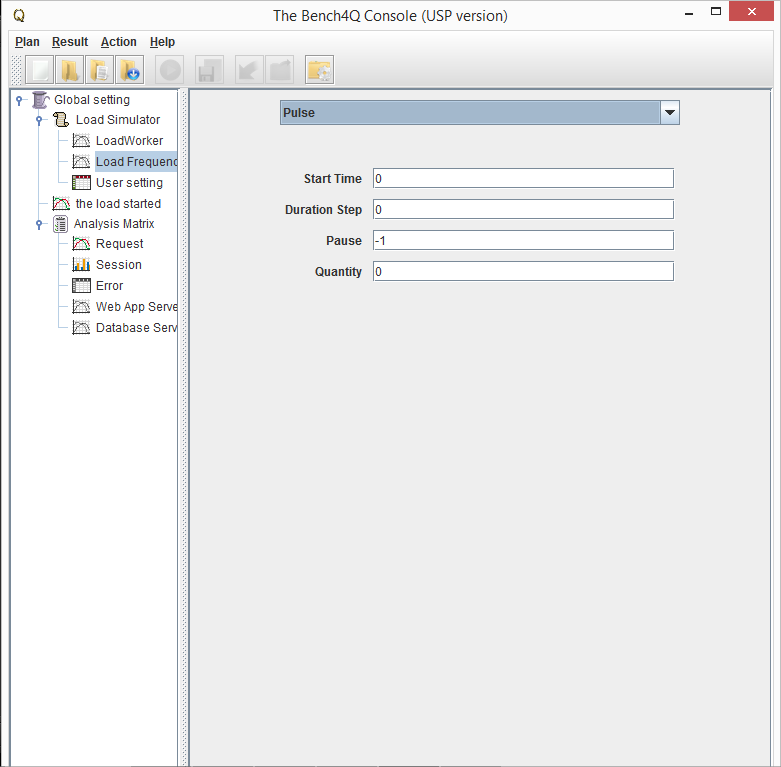
\includegraphics[scale=0.6]{console-bench4Q-usp.png}
	\caption{Console de programação de carga de trabalho.}
	\label{fig:interface-criada-beanch4q}
	\fautor
\end{figure}


\section{Teste de modulação}

A carga de trabalho é imposta ao sistema por meio de requisições HTTP enviadas pelos EBs ao SUT que são executadas nos servidores de aplicação das máquinas virtuais instanciadas no \textit{host}. Essas requisições exigem que as máquinas virtuais se ocupem pelo tempo necessário para processá-las, alterando o desempenho experimentado pelo sistema.
Segundo \citeonline{Nobile2013}, existem dois fatores associados a uma requisição e que afetam diretamente o desempenho do sistema:
%\begin{citacao}
o tempo de processamento e a quantidade de carga imposta pelas requisições, são dados pelo tempo de processamento e pela taxa de chegada de novas requisições, respectivamente. Com o tempo, a quantidade e o tamanho das requisições podem se alterar, dependendo do perfil de utilização dos usuários que utilizam o serviço naquele momento. Havendo um aumento em algum desses fatores é possível que o desempenho do sistema sofra degradação, podendo, em casos extremos, entrar em colapso.
%\end{citacao}

É possível informar previamente a execução os parâmetros da modulação. Por exemplo, ao escolher a opção degrau, é necessário informar quantos EBs geram o degrau, em que instante de tempo, e qual o tempo de duração e por fim qual a sua polaridade (com base em um pulso elétrico a positiva sairia de zero e chega a um, a negativa, sairia de um e chegaria a zero), é possível obter resultados conforme a Figura \ref{fig:grafico-carga-modulada-teste}.

\begin{figure}[!htb]
	\centering
	\begin{subfigure}{\linewidth}
		\centering
		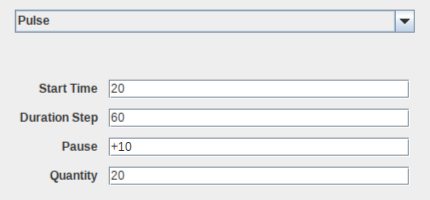
\includegraphics[scale=0.7]{condiguracao-carga-modulada1.png}
		\caption{Teste de configuração da carga a ser modulada}
		\label{fig:configuracao-carga-modulada-teste}
	\end{subfigure}
	
	\begin{subfigure}{\linewidth}
		\centering
		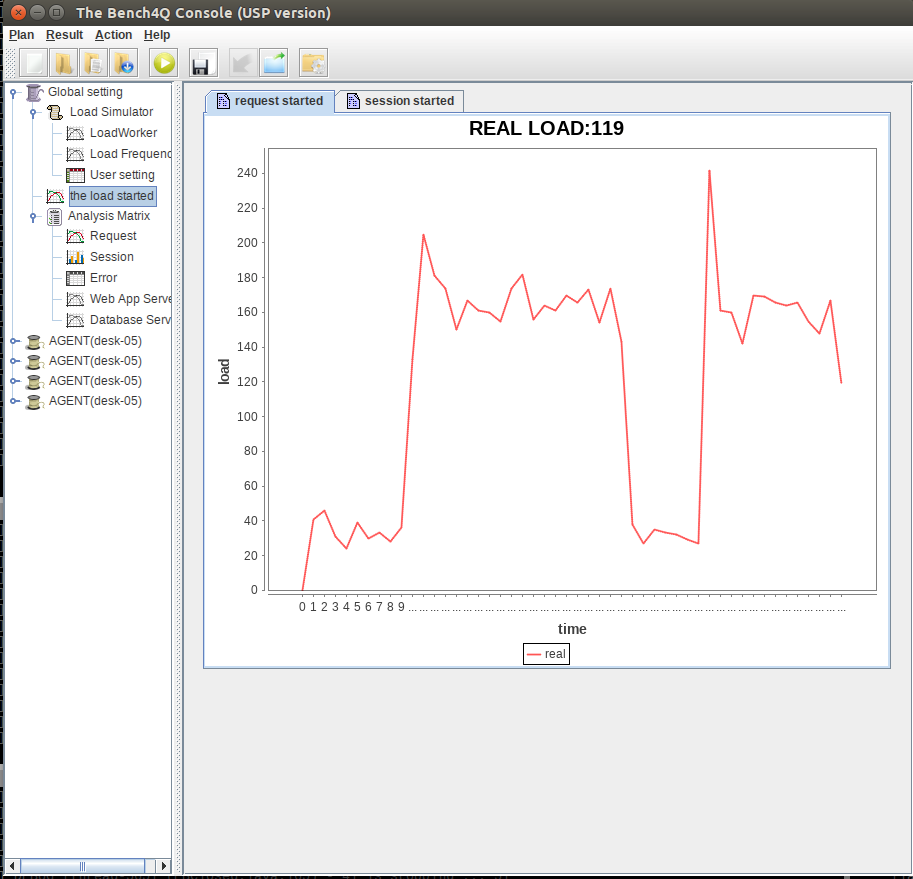
\includegraphics[scale=0.6]{grafico-carga-modulada-teste.png}
		\caption{Carga gerada com base na configuração teste}
		\label{fig:grafico-carga-modulada-teste}
	\end{subfigure}  
	\caption{Teste de modulação da carga}  
	\label{fig:carga-modulada-teste}
	\fautor
\end{figure}  

A Figura \ref{fig:carga-modulada-teste} ilustra uma carga teste modulada já pela extensão. A figura \ref{fig:configuracao-carga-modulada-teste} apresenta os parâmetros utilizado para fazer o teste. A carga modulada atuará a partir do 10º segundo de experimentação e com uma duração de 20 segundos; com 30 segundos de experimentação ocorrerá uma pausa de 7 segundos e um novo degrau será gerado em seguida, o qual se manterá até o final do experimento. Para este exemplo foram fixados 40 EBs para modular o comportamento da carga. Este comportamento pode ser apreciado no item \ref{fig:grafico-carga-modulada-teste} da mesma figura \ref{fig:carga-modulada-teste}. Vale salientar que o gráfico gerado e apresentado na figura \ref{fig:carga-modulada-teste} de item \ref{fig:grafico-carga-modulada-teste}, é uma característica nativa ao \textit{benchmark}.



O Bench4Q, possui uma documentação sobre a ferramenta. Devido a extensão do \textit{benchmark} foi elaborada uma documentação seguindo os padrões da última versão original e esta pode ser conferida no apêndice \ref{chapter:documentacao} que traz informações do programa e qual seu objetivo, entradas suportadas e saídas esperadas, exemplo de como executar o programa e tabela descrevendo as principais características do mesmo.

%O Bench4Q também não suporta nativamente a alocação e a deslocação dos recursos em tempo de simulação. Um conjunto de implementações foi necessário para estender o \textit{benchmark}.%, essas aplicações não lidam com a modulação da carga de trabalho, mas manipulação a distribuição da carga de trabalho em um conjunto de servidores, da mesma maneira que um ambiente de nuvem, assim como o gerenciamento dos recursos da proposta de arquitetura. Contudo, os detalhes dessa implementação não serão apresentados e discutidos neste trabalho, uma vez este contexto foge do foco e da proposta do trabalho que tem por objetivo a modulação da carga.

